%Đây là template dùng cho đề cương đề tài tốt nghiệp
%Khoa Công nghệ Thông tin
%Trường Đại học Khoa học Tự nhiên, ĐHQG-HCM

%Liên hệ về mẫu LaTEX này: Thầy Bùi Huy Thông (bhthong@fit.hcmus.edu.vn)

\documentclass{article}[14pt]
\usepackage[utf8]{vietnam}
\usepackage{enumerate}
\usepackage{enumitem}
\usepackage{multicol}
\usepackage{listings}
\usepackage[left=2cm,right=2cm,top=2.5cm,bottom=2.5cm]{geometry}
\usepackage{verbatim}
\usepackage{graphicx}
\usepackage{url}
\usepackage{fancyhdr}
\usepackage{fancybox,framed}
\linespread{1.3}
\usepackage{lastpage}
\usepackage{floatrow}
\usepackage{floatrow}
\usepackage[utf8]{inputenc}
\usepackage{array}
\usepackage{longtable}
\usepackage{geometry}
\geometry{a4paper, margin=1in}
\pagenumbering{arabic}
%\pagestyle{fancy}
\newfloatcommand{capbtabbox}{table}[][\FBwidth]
\usepackage{caption}
\captionsetup[figure]{font=large} 
\usepackage{blindtext}
\usepackage{titlesec}
\usepackage[nottoc]{tocbibind}


\usepackage{array} % Gói cần thiết cho kiểu cột m{}



\titleformat*{\section}{\LARGE\bfseries}
\titleformat*{\subsection}{\Large\bfseries}
\titleformat*{\subsubsection}{\large\bfseries}
%\addbibresource{ref.bib}


\begin{document}
    \begin{figure}[h]
        \begin{floatrow}
        \ffigbox{
\includegraphics[scale = .4]{logo.png}}  
        {%
    
        }
        \capbtabbox{
            \begin{tabular}{l}
            \multicolumn{1}{c}{\textbf{\begin{tabular}[c]{@{}c@{}}TRƯỜNG ĐẠI HỌC KHOA HỌC TỰ NHIÊN\\KHOA CÔNG NGHỆ THÔNG TIN\end{tabular}}} \\ \\ \\
            \end{tabular}
        }
        {%
    
        }
        \end{floatrow}
    \end{figure}
    
    \begin{center}
        
        %Xác định loại đề tài tốt nghiệp tương ứng: Khóa luận, Thực tập, Đồ án
        \textbf{\Large LUẬN VĂN \\  TỐT NGHIỆP} \\ 
    \end{center}
    
    %\vspace{.5cm}
    
    \begin{center}
    %Tên đề tài phải VIẾT HOA
        
        \textbf{\huge Hệ quản trị cơ sở dữ liệu quan hệ phân tán hỗ trợ xử lý dữ liệu lớn trực tuyến } 
        \\
        
    %Tên đề tài bằng tiếng Anh (nếu có)
    \vspace{.5cm}
        \textit{\textbf{\Large (Distributed Relational Database Management System Supporting Online Big Data Processing  )}}
    \end{center}
    
    \vspace{.5cm}
    
    \Large
    \section{THÔNG TIN CHUNG}
    \begin{itemize}[label = {}]
        
        \item \textbf{Người hướng dẫn:} 
        %Thể hiện dạng: <Chức danh> <Họ và tên> (<Đơn vị công tác>)
        \begin{itemize}
            \item TS. Ngô Huy Biên (Khoa Công nghệ Thông tin)
        \end{itemize}{}
    
        
        \item \textbf{Học viên thực hiện:}
        
        %Thể hiện dạng: <Họ và tên sinh viên> (MSSV: )
        \begin{itemize}
        
            \item Trần Hữu Nghĩa (MSSV: 21C12005) 
           
        \end{itemize}

       %Chọn loại thích hợp
        \item \textbf{Mã số ngành:} 8480104
        
        \item \textbf{Thời gian thực hiện:} Từ \textit{06/2023} đến \textit{12/2024}
        
        
    \end{itemize}
    
    \pagebreak 

   
    \begin{figure}[h]
        \begin{floatrow}
        \ffigbox{
\includegraphics[scale = .4]{logo.png}}  
        {%
    
        }
        \capbtabbox{
            \begin{tabular}{l}
            \multicolumn{1}{c}{\textbf{\begin{tabular}[c]{@{}c@{}}TRƯỜNG ĐẠI HỌC KHOA HỌC TỰ NHIÊN\\KHOA CÔNG NGHỆ THÔNG TIN\end{tabular}}} \\ \\ \\
            \end{tabular}
        }
        {%
    
        }
        \end{floatrow}
    \end{figure}
    
    \begin{center}
        
        %Xác định loại đề tài tốt nghiệp tương ứng: Khóa luận, Thực tập, Đồ án
        \textbf{\Large ĐỀ CƯƠNG LUẬN VĂN \\  TỐT NGHIỆP} \\ 
    \end{center}
    
    %\vspace{.5cm}
    
    \begin{center}
    %Tên đề tài phải VIẾT HOA
        
        \textbf{\huge Hệ quản trị cơ sở dữ liệu quan hệ phân tán hỗ trợ xử lý dữ liệu lớn trực tuyến } 
        \\
        
    %Tên đề tài bằng tiếng Anh (nếu có)
    \vspace{.5cm}
        \textit{\textbf{\Large (Distributed Relational Database Management System Supporting Online Big Data Processing  )}}
    \end{center}
    
    \vspace{.5cm}
    
    \Large
    \section{THÔNG TIN CHUNG}
    \begin{itemize}[label = {}]
        
        \item \textbf{Người hướng dẫn:} 
        %Thể hiện dạng: <Chức danh> <Họ và tên> (<Đơn vị công tác>)
        \begin{itemize}
            \item TS. Ngô Huy Biên (Khoa Công nghệ Thông tin)
        \end{itemize}{}
    
        
        \item \textbf{Học viên thực hiện:}
        
        %Thể hiện dạng: <Họ và tên sinh viên> (MSSV: )
        \begin{itemize}
        
            \item Trần Hữu Nghĩa (MSSV: 21C12005) 
           
        \end{itemize}

       %Chọn loại thích hợp
        \item \textbf{Mã số ngành:} 8480104
        
        \item \textbf{Thời gian thực hiện:} Từ \textit{06/2023} đến \textit{12/2024}
        
        
    \end{itemize}
    
    \pagebreak 
    
    \section{NỘI DUNG THỰC HIỆN}
    {

    %Mỗi mục dưới đây phải viết ít nhất là 5 câu mô tả/giới thiệu.
    
    \subsection{Giới thiệu tổng quan }
    
Các hệ thống cơ sở dữ liệu quan hệ truyền thống gặp khó khăn trong việc xử lý dữ liệu lớn khi thực hiện các hoạt động OLAP (Online Analytical Processing) do khả năng mở rộng hạn chế và hiệu suất truy vấn không tốt. Việc mở rộng hệ thống cơ sở dữ liệu để đáp ứng nhu cầu tăng lên của người dùng và dữ liệu có thể là một thách thức lớn. Một số hệ thống không hỗ trợ mở rộng theo cả hai chiều (scale-up và scale-out), điều này có thể hạn chế khả năng của tổ chức để mở rộng hệ thống của họ khi cần dẫn đến thời gian phản hồi truy vấn chậm và lãng phí tài nguyên (như bộ vi xử lý, bộ nhớ).


Apache Hive\cite{aluko2019big}, một hệ thống dữ liệu lớn phân tán dựa trên Hadoop, được thiết kế để xử lý và phân tích dữ liệu lớn bằng ngôn ngữ truy vấn giống SQL (HiveQL). Hive không phải là một hệ thống cơ sở dữ liệu thời gian thực, mà chủ yếu tập trung vào việc cung cấp khả năng phân tích dữ liệu lớn với độ trễ cao hơn. Hive sử dụng Hadoop MapReduce để thực hiện các truy vấn và chạy trên HDFS (Hadoop Distributed File System), cho phép phân tán và lưu trữ dữ liệu trên nhiều máy chủ. Tuy nhiên, Hive mang đến một số hạn chế. Độ trễ cao trong việc xử lý dữ liệu, khả năng tối ưu hóa truy vấn không mạnh mẽ, và dù hoạt động tốt trên hệ thống phân tán.

Tiếp theo là Spark SQL\cite{armbrust2015spark}, một thành phần của Apache Spark, đã khắc phục được một số nhược điểm của Hive. Spark SQL tận dụng công nghệ xử lý song song của Spark, giúp cải thiện hiệu suất và khả năng mở rộng, làm giảm thời gian truy vấn so với Hive. Nó sử dụng Catalyst Optimizer, một framework tối ưu hóa truy vấn mạnh mẽ, hỗ trợ xử lý dữ liệu cấu trúc và bán cấu trúc, và tương thích với Hive cũng như Hadoop, làm nó mở rộng khả năng tương tác với nhiều nguồn dữ liệu.

Bên cạnh Hive và Spark SQL, Greenplum\footnote{https://greenplum.org} cũng đóng một vai trò quan trọng trong lĩnh vực xử lý dữ liệu lớn. Greenplum là một hệ cơ sở dữ liệu Massively Parallel Processing (MPP) dựa trên PostgreSQL, một hệ thống quản lý cơ sở dữ liệu quan hệ mã nguồn mở. Nó được phát triển để xử lý khối lượng công việc dữ liệu quy mô lớn, dành riêng cho các ứng dụng phân tích, học máy và trí tuệ nhân tạo. Điều này giúp Greenplum cung cấp một số lợi ích mà Hive và SparkSQL không thể cung cấp, bao gồm khả năng quản lý và truy vấn hiệu quả petabytes dữ liệu theo cách phân tán.


Jason Arnold cùng các cộng sự đã đề xuất giải pháp có tên là “A High-Performance Distributed Relational Database System for Scalable OLAP Processing (HRDBMS)\cite{arnold2019hrdbms}. Nhận thấy những ưu điểm vượt trội và tiềm năng của giải pháp HRDBMS, luận văn này quyết định tập trung nghiên cứu và cài đặt giải pháp "tối ưu hóa truy vấn trên dữ liệu lớn" dựa trên các đề xuất của Jason Arnold.

HRDBMS với kiến trúc phân tán và khả năng xử lý song song, mang lại hiệu suất cao và linh hoạt khi thực hiện các truy vấn OLAP trên dữ liệu lớn. Nó cũng cho phép mở rộng khả năng xử lý truy vấn mà không làm giảm hiệu suất, một điều mà các hệ thống Hive, SparkSQL và Greenplum không thể đạt được hoàn toàn. Bằng việc tận dụng những khả năng này, luận văn hy vọng sẽ cung cấp một giải pháp tối ưu để tăng cường hiệu suất truy vấn trên dữ liệu lớn.

Mục tiêu chính của nghiên cứu này là khai thác, thử nghiệm và đánh giá hiệu năng của mã nguồn cùng các kỹ thuật trong hệ thống HRDBMS được trình bày trong công trình HRDBMS. Điều này nhằm xây dựng một hệ thống quản lý cơ sở dữ liệu hiệu năng cao, sánh ngang với các hệ thống MPP và có khả năng mở rộng tương đương với các nền tảng Big Data. Cụ thể như sau:

Thử nghiệm mã nguồn và áp dụng kỹ thuật: Tiến hành thử nghiệm mã nguồn và áp dụng các kỹ thuật của hệ thống HRDBMS, nhằm đánh giá hiệu quả và khả năng mở rộng của hệ thống trong thực tế.

Nghiên cứu hiệu năng trên mỗi node: Phân tích hiệu năng của hệ thống HRDBMS trên mỗi node, đánh giá sự phân tán và tính song song của hệ thống trong việc xử lý các truy vấn OLAP.

Đề xuất các phương pháp cải tiến và tối ưu hóa: Dựa trên kết quả thử nghiệm và đánh giá, đề xuất các phương pháp cải tiến và tối ưu hóa hệ thống HRDBMS, giúp nâng cao hiệu năng và khả năng mở rộng trong việc xử lý OLAP.
So sánh với các hệ thống MPP và nền tảng Big Data đối chiếu hiệu năng và khả năng mở rộng của hệ thống HRDBMS với các hệ thống MPP và nền tảng Big Data, nhằm xác định ưu nhược điểm của mỗi hệ thống trong việc xử lý dữ liệu lớn.

Qua việc thử nghiệm mã nguồn và áp dụng các kỹ thuật của hệ thống HRDBMS, đánh giá và nghiên cứu hiệu quả của các kỹ thuật này trong thực tế, đồng thời tìm hiểu về khả năng mở rộng của hệ thống và hiệu năng trên mỗi node. Mục tiêu cuối cùng là đề xuất các phương pháp cải tiến và tối ưu hóa hệ thống dựa trên những kết quả đạt được, nhằm mang lại giải pháp hiệu quả hơn cho việc xử lý OLAP trong các hệ thống cơ sở dữ liệu hiện đại.

\subsection{Mục đích nghiên cứu }

Nghiên cứu này tập trung vào việc phát triển một giải pháp tiên tiến để đương đầu với những thách thức tăng lên không ngừng từ việc quản lý và xử lý lượng dữ liệu lớn. Ngày nay, việc xử lý dữ liệu lớn đang trở thành một nhiệm vụ phức tạp, yêu cầu sự linh hoạt và hiệu suất tối ưu trong việc quản lý tài nguyên và truy vấn dữ liệu.

Vì vậy, mục tiêu chính của nghiên cứu này là xây dựng một hệ thống cơ sở dữ liệu phân tán, sử dụng các phương pháp tiên tiến. Nghiên cứu sẽ đánh giá tính khả thi và hiệu suất của hệ thống này trong việc xử lý và quản lý dữ liệu lớn.

Kết quả của nghiên cứu này sẽ mang lại những lợi ích thiết thực và giá trị đáng kể, đặc biệt cho những doanh nghiệp vừa và lớn trong lĩnh vực thương mại điện tử và bán lẻ và các cửa hàng bán lẻ vừa và nhỏ khác. Các tổ chức này hàng ngày phải tạo ra và xử lý một lượng lớn dữ liệu. Quản lý và tối ưu hóa quá trình này, họ cần một hệ thống quản lý dữ liệu hiệu quả và linh hoạt. Đáp ứng nhu cầu này, HRDBMS, trở thành lựa chọn tối ưu với các tính năng mạnh mẽ của mình.

HRDBMS, dựa trên mô hình Massively Parallel Processing (MPP), có khả năng xử lý dữ liệu lớn và phức tạp một cách nhanh chóng, hiệu quả và đáng tin cậy một yếu tố cần thiết cho các doanh nghiệp kỷ nguyên số hiện đại.

HRDBMS có những đặc trưng sau:

\begin{itemize}
\item \textbf{Bộ tối ưu hóa truy vấn dựa trên chi phí (A cost-based query optimizer):} HRDBMS sử dụng kỹ thuật tối ưu hóa truy vấn tiên tiến, giúp nâng cao hiệu suất của các truy vấn trên dữ liệu lớn.
\item \textbf{Môi trường thực thi song song và phân tán hoàn toàn: }Điều này giúp HRDBMS tận dụng lợi thế về khả năng mở rộng của các nền tảng Big Data.
\item \textbf{Hỗ trợ cấu trúc chỉ mục: }Điều này giúp tăng tốc độ truy vấn bằng cách giảm bớt số lượng dữ liệu cần phải quét.
\item \textbf{Quản lý bộ đệm tự động:} HRDBMS sử dụng cơ chế quản lý bộ đệm truyền thống để tăng hiệu suất của các truy vấn.
\item \textbf{Hỗ trợ giao dịch: }HRDBMS cung cấp cơ chế giao dịch đảm bảo tính nhất quán và độ tin cậy của dữ liệu.
\item \textbf{T\textbf{hực hiện shuffle không chặn:} }Điều này giúp tăng hiệu suất của các truy vấn phức tạp yêu cầu hoán đổi dữ liệu giữa các nút.
\item \textbf{Hỗ trợ phân vùng ngang:} Điều này cho phép HRDBMS tận dụng cấu trúc phân vùng dữ liệu để tăng hiệu suất truy vấn.
\end{itemize}

Như vậy, HRDBMS là một giải pháp lý tưởng cho các doanh nghiệp vừa và lớn trong lĩnh vực thương mại điện tử và bán lẻ và các cửa hàng bán lẻ vừa và nhỏ khác, giúp họ nâng cao chất lượng dịch vụ và trải nghiệm của khách hàng trong môi trường thương mại điện tử ngày càng cạnh tranh.

\subsection{Đối tượng nghiên cứu }

Nghiên cứu và cài đặt hệ thống quản lý cơ sở dữ liệu (Database Management System) với mỗi node có hiệu suất tương đương cơ sở dữ liệu Massively Parallel Processing (MPP) đồng thời có khả năng mở rộng tương đương với các nển tảng Big Data như Hadoop, Spark. Bao gồm mã nguồn do Jason Arnold đề xuất và cung cấp\footnote{https://github.com/IITDBGroup/HRDBMS}.
Kiến trúc của hệ thống như hình \ref{fig:Component}.

\begin{figure}[htbp]
\centerline{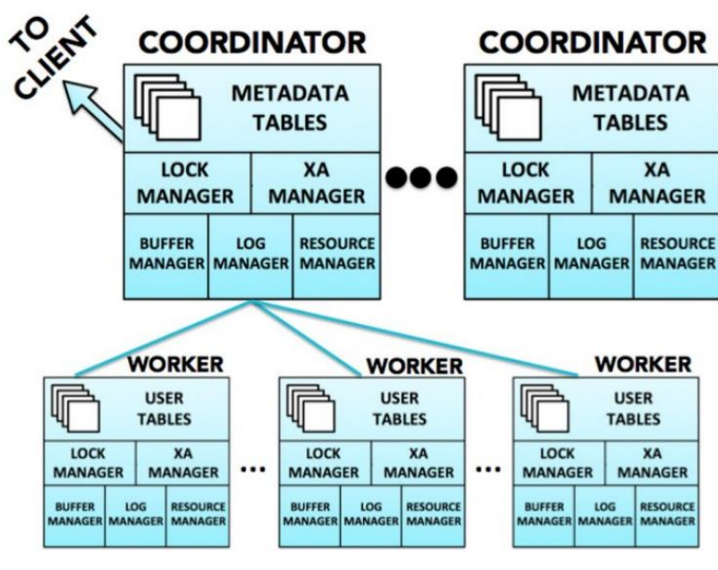
\includegraphics[scale=.7]{images/Component.png}}
\captionsetup{font=Large}
\caption{Kiến trúc hệ thống \cite{arnold2019hrdbms}}
\label{fig:Component}
\end{figure}

Kiến trúc của hệ thống HRDBMS gồm 2 thành phần chính là: worker và coordinator:
Coordinator đảm nhiệm vai trò giao tiếp với người dùng (client), chịu trách nghiệm tối ưu truy vấn. quản lý tài nguyên trên toàn cụm (cluster), phân phối giao dịch (Transaction coordination) đảm bảo tính nhất quán của các giao dịch (transaction).

Worker đảm nhiệm vai trò lưu trữ dữ liệu và thực thi các truy vấn nhận từ Coordinator. 

Quy trình mà giải pháp sẽ cài đặt: Client (người dùng) gửi sql command cho Coordinator. Coordinator sẽ giao tác vụ (task) cho các worker dựa vào dữ liệu mà chúng đang lưu trữ. Worker thực hiện truy vấn mà chúng đang lưu trữ sau khi hoàn thành gửi kết quả truy vấn cho Coordinator. Coordiantor tổng hợp kết quả gữi từ các woker và trả kết quả cuối cùng cho người dùng như hình \ref{fig:diagramworkflow}.

\begin{figure}[htbp]
\centerline{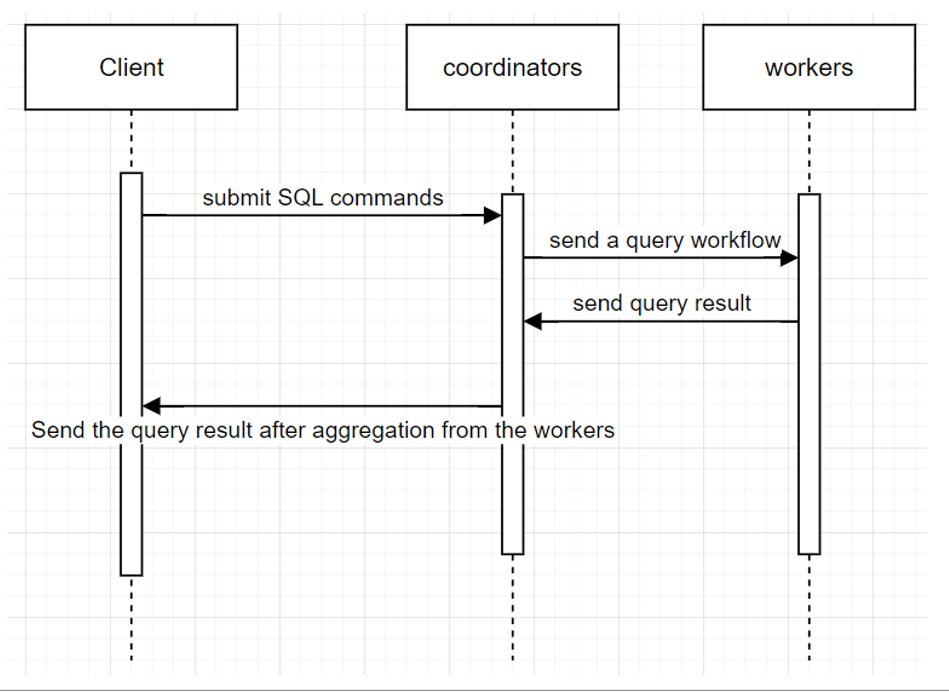
\includegraphics[scale=.7]{images/diagramworkflow.png}}
\captionsetup{font=Large}
\caption{Quy trình tối ưu truy vấn}
\label{fig:diagramworkflow}
\end{figure}

Quy trình này giúp tận dụng sức mạnh của nhiều máy chủ để xử lý dữ liệu và truy vấn một cách song song và hiệu quả hơn.
Quá trình tối ưu truy vấn trong HRDBMS gồm 3 giai đoạn

Giai đoạn 1 Global Optimization như hình \ref{fig:phase1}
“Global Optimization là một giai đoạn trong quá trình tối ưu hóa truy vấn trong hệ thống cơ sở dữ liệu\cite{arnold2019hrdbms}. Trong giai đoạn này, các phép tối ưu hóa sử dụng hai phương pháp: heuristic và cost-based.

Heuristic optimization là phương pháp sử dụng các quy tắc, kinh nghiệm và giải thuật đơn giản để tối ưu hóa truy vấn. Chẳng hạn như, phương pháp đặt bảng nhỏ trước, chọn giá trị được lặp lại ít nhất cho điều kiện WHERE, ...

Cost-based optimization là phương pháp sử dụng các thống kê và mô hình tính toán chi phí để đánh giá và so sánh các kế hoạch truy vấn khác nhau. Nó sẽ lựa chọn kế hoạch truy vấn có chi phí thấp nhất.

Trong giai đoạn này, tối ưu hóa truy vấn sẽ được thực hiện mà không quan tâm đến việc phân phối dữ liệu trên các node trong hệ thống phân tán. Giai đoạn này thường sử dụng trước khi thực hiện phân phối dữ liệu và thực hiện tối ưu hóa cục bộ trên mỗi node trong hệ thống.

“HRDBMS giảm số lần truy cập vào dữ liệu trong các truy vấn lồng nhau (de-correlate and un-nest). Sau đó áp dụng một số biến thể của thuật toán có tên là greedy join enumeration\cite{arnold2019hrdbms}. HRDBMS sử dụng thống kê để ước tính số hàng sẽ được đầu ra bởi mỗi khả năng join. Sau đó, nó sắp xếp các join theo cách cố gắng giảm thiểu tổng số hàng được xử lý bởi mỗi lần join vẫn cho ra kết quả chính xác.

\begin{figure}[htbp]
\centering
\makebox[\linewidth]{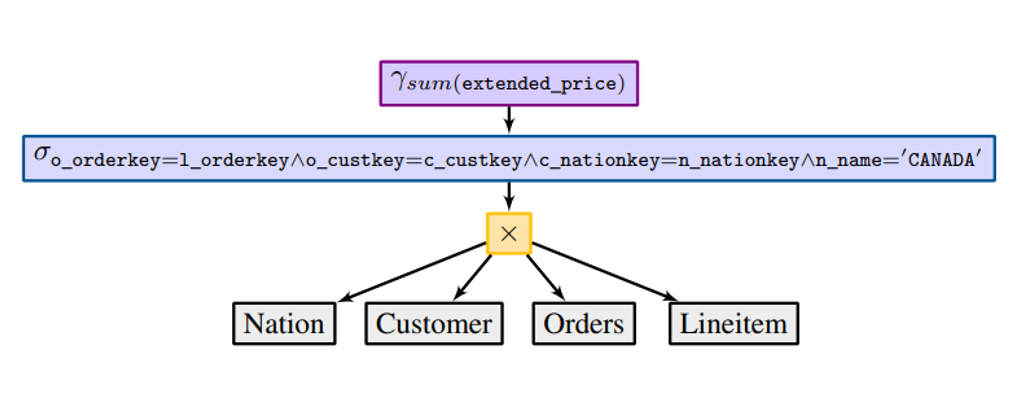
\includegraphics[width=1.3\textwidth,keepaspectratio]{images/phase1.png}}
\captionsetup{font=Large}
\caption{Kế hoạch truy vấn ban đầu \cite{arnold2019hrdbms}}
\label{fig:phase1}
\end{figure}

HRDBMS sử dụng left-deep như hình \ref{fig:phase2}  là một kiểu kế hoạch truy vấn trong hệ thống cơ sở dữ liệu quan hệ. Các bảng được kết nối từ trái sang phải theo thứ tự liên tiếp. như hình bên dưới ta thấy được nation và customer được join đầu tiên sau đó tới orders cuối cùng tới lineitem.

\begin{figure}[htbp]
\centering
\makebox[\linewidth]{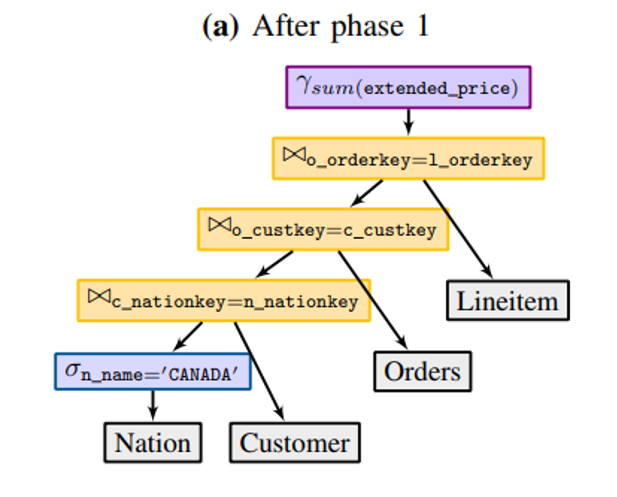
\includegraphics[width=1.3\textwidth,keepaspectratio]{images/phase2.png}}
\captionsetup{font=Large}
\caption{Kế hoạch tối ưu truy vấn của giai đoạn đầu tiên \cite{arnold2019hrdbms}}
\label{fig:phase2}
\end{figure}

Giai đoạn 2 Dataflow Conversion 
“Giai đoạn này là cây toán tử (operator tree) được chuyển thành dòng dữ liệu phân tán(distributed dataflow) đơn giản bằng cách chia mỗi toán tử quét riêng lẻ cho từng phân đoạn(fragment) dựa trên điều kiện truy vấn” \cite{arnold2019hrdbms}. Phân đoạn là một phần của bảng dữ liệu, được chia nhỏ và lưu trữ trên các woker khác nhau trong cụm phân tán việc này giúp xử lý và truy vấn dữ liệu trở nên dễ dàng hơn và hiệu quả hơn như hình \ref{fig:phase3}. 

\begin{figure}[htbp]
\centering
\makebox[\linewidth]{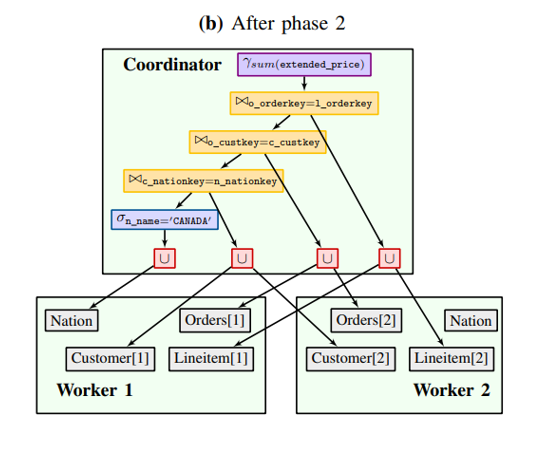
\includegraphics[width=1.3\textwidth,keepaspectratio]{images/phase3.png}}
\captionsetup{font=Large}
\caption{Biểu đồ dòng dữ liệu được tạo ra \cite{arnold2019hrdbms}}
\label{fig:phase3}
\end{figure}

Giai đoạn 3 Dataflow Optimization 
“Trong giai đoạn này sẽ phân chia lại công việc từ Coordiantor sẽ giao cho các Woker” như hình \ref{fig:phase4}. Mục đích của việc này là tận dụng các phân đoạn đã được lưu trong worker để giảm lượng giao tiếp không cần thiết. Việc còn lại của Coordinator là tổng hợp lại kết quả từ các worker gửi về và trả kết quả cho client.


\begin{figure}[htbp]
\centering
\makebox[\linewidth]{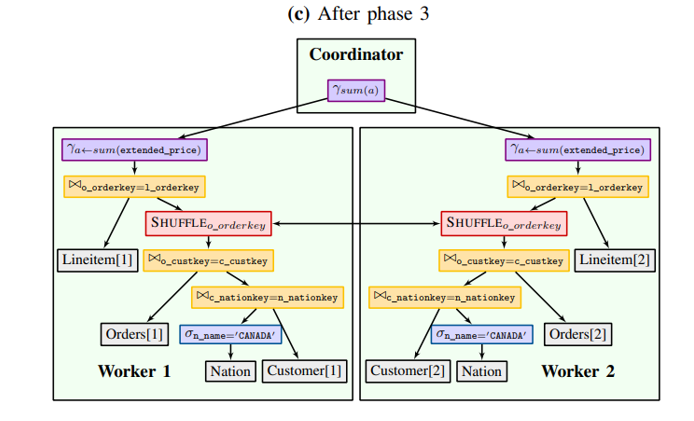
\includegraphics[width=1.3\textwidth,keepaspectratio]{images/phase4.png}}
\captionsetup{font=Large}
\caption{Giai đoạn tối ưu hóa cuối cùng \cite{arnold2019hrdbms}}
\label{fig:phase4}
\end{figure}




Để đánh giá hiệu quả và tiềm năng của giải pháp, luận văn dự kiến sẽ so sánh giải pháp với các cơ sở dữ liệu Apache Hive\footnote{https://hive.apache.org/general/downloads} , Spark SQL\footnote{https://spark.apache.org/downloads.html}, Greenplum\footnote{https://github.com/greenplum-db/gpdb/releases}  độ đo hiệu suất (performance) và khả năng mở rộng (scalability). Cụ thể sẽ sử dụng độ đo TPC-H. TPC-H là một bộ chuẩn kiểm tra hiệu suất (benchmark) cho các hệ thống cơ sở dữ liệu. TPC-H được thiết kế để đánh giá hiệu năng của các hệ thống cơ sở dữ liệu trong việc xử lý các truy vấn phức tạp, chủ yếu liên quan đến các tác vụ OLAP (Online Analytical Processing). TPC-H gồm 22 truy vấn chuẩn và một tập dữ liệu tổng hợp được tạo ra dựa trên mô hình dữ liệu quan hệ với 8 bảng (PART, SUPPLIER, PARTSUPP, CUSTOMER, ORDERS, LINEITEM, NATION, và REGION)\footnote{\url{https://www.tpc.org/TPC_Documents_Current_Versions/pdf/TPC-H_v3.0.1.pdf}}.
Cụ thể để đánh giá hiệu suất của một hệ thống cơ sở dữ liệu thực hiện các bước sau:

\textbf{Tải về và cài đặt TPC-H:} Truy cập trang chủ của TPC-H\footnote{https://www.tpc.org/TPC\_Documents\_Current\_Versions/download\_programs/tools-download-request5.asp} để tải về mã nguồn.

\textbf{Tạo cơ sở dữ liệu:} Trên hệ thống tạo một cơ sở dữ liệu mới để chứa dữ liệu TPC-H.

\textbf{Tạo bảng và khóa ngoại: }Dựa trên định nghĩa của TPC-H, sử dụng lệnh SQL để tạo các bảng (CUSTOMER, SUPPLIER, PART, PARTSUPP, REGION, NATION, ORDERS, LINEITEM)  và khóa ngoại tương ứng.

\textbf{Sinh dữ liệu: }Trong thư mục chứa mã nguồn TPC-H, biên dịch và xây dựng công cụ dbgen theo hướng dẫn. Sử dụng dbgen để sinh dữ liệu mẫu cho các bảng. Thay đổi thông số SF (Scale Factor) để điều chỉnh kích thước dữ liệu.Các tệp dữ liệu được sinh ra sẽ có định dạng “.tbl”.

\textbf{Nạp dữ liệu vào cơ sở dữ liệu: }Import dữ liệu từ các tệp .tbl vào các bảng tương ứng trong cơ sở dữ liệu. 

\textbf{Sinh truy vấn:} Sử dụng qgen để sinh truy vấn mẫu cho TPC-H. Thông tin 22 truy vấn 

\begin{itemize}
\item Truy vấn 1 (Pricing Summary Report Query): Tính toán một báo cáo giá cả tổng hợp cho các dòng sản phẩm trong một khoảng thời gian nhất định.
\item Truy vấn 2 (Minimum Cost Supplier Query): Tìm nhà cung cấp có chi phí nhỏ nhất cho mỗi sản phẩm trong một quốc gia.
\item Truy vấn 3 (Shipping Priority Query): Tìm 10 đơn hàng lớn nhất chưa được giao trong một khoảng thời gian nhất định.
\item Truy vấn 4 (Order Priority Checking Query): Đếm số lượng đơn hàng chưa được giao trong mỗi loại ưu tiên.
\item Truy vấn 5 (Local Supplier Volume Query): Tính tổng giá trị đơn hàng của các nhà cung cấp địa phương trong mỗi quốc gia.
\item Truy vấn 6 (Forecasting Revenue Change Query): Dự đoán doanh thu thay đổi dựa trên việc áp dụng một chiết khấu nhất định cho các đơn hàng trong một khoảng thời gian nhất định.
\item Truy vấn 7 (Volume Shipping Query): Tính tổng giá trị đơn hàng giữa các quốc gia trong một khoảng thời gian nhất định.
\item Truy vấn 8 (National Market Share Query): Tính tổng giá trị đơn hàng của một phân khúc thị trường trong một quốc gia nhất định.

Truy vấn 9 (Product Type Profit Measure Query): Tính lợi nhuận của một loại sản phẩm nhất định trong một khoảng thời gian nhất định.
\item Truy vấn 10 (Returned Item Reporting Query): Báo cáo các mặt hàng bị trả lại trong một khoảng thời gian nhất định.
\item Truy vấn 11 (Important Stock Identification Query): Xác định các sản phẩm quan trọng có tồn kho lớn hơn một giá trị nhất định.
\item Truy vấn 12 (Shipping Modes and Order Priority Query): Đánh giá tỷ lệ các phương thức vận chuyển và mức độ ưu tiên của đơn hàng trong một khoảng thời gian nhất định.
\item Truy vấn 13 (Customer Distribution Query): Đếm số lượng khách hàng có lượng đơn hàng trong một khoảng nhất định.
\item Truy vấn 14 (Promotion Effect Query): Tính tỷ lệ doanh thu khuyến mãi so với tổng doanh thu trong một khoảng thời gian nhất định.
\item Truy vấn 15 (Top Supplier Query): Xác định nhà cung cấp hàng đầu dựa trên tổng giá trị đơn hàng.

\item Truy vấn 16 (Parts/Supplier Relationship Query): Đếm số lượng nhà cung cấp cung cấp các bộ phận phù hợp với điều kiện nhất định.
\item Truy vấn 17 (Small-Quantity-Order Revenue Query): Tính tổng doanh thu cho các đơn hàng có số lượng sản phẩm nhỏ hơn mức trung bình của một loại sản phẩm nhất định.
\item Truy vấn 18 (Large-Volume-Customer Query): Liệt kê các đơn hàng có giá trị lớn hơn một ngưỡng nhất định của những khách hàng mua nhiều.
\item Truy vấn 19 (Discounted Revenue Query): Tính tổng doanh thu cho các đơn hàng có chiết khấu nằm trong một khoảng nhất định và số lượng sản phẩm nằm trong một khoảng nhất định.
\item Truy vấn 20 (Potential Part Promotion Query): Tìm các nhà cung cấp tiềm năng có thể cung cấp các bộ phận phù hợp với điều kiện nhất định trong một chiến dịch khuyến mãi.
\item Truy vấn 21 (Supplier's Unfulfilled Orders Query): Xác định các nhà cung cấp mà tỷ lệ đơn hàng chưa được thực hiện lớn hơn một ngưỡng nhất định.
\item Truy vấn 22 (Global Sales Opportunity Query): Đếm số lượng khách hàng có tổng giá trị đơn hàng nằm trong một khoảng giá trị nhất định.
    
\end{itemize}


\textbf{Chạy các truy vấn TPC-H:} Thực thi lần lượt các truy vấn TPC-H trên hệ thống DBMS. Ghi lại thời gian chạy cho mỗi truy vấn.

\textbf{Tính toán và phân tích kết quả:} So sánh kết quả hiệu năng của hệ thống DBMS với các giá trị tham chiếu từ TPC-H hoặc với kết quả của các hệ thống khác để đánh giá hiệu suất của hệ thống DBMS.

Để đánh giá hiệu suất của hệ thống dự kiến thực hiện trên 8 node sử dụng môi trường AWS(Amazon Web Services) EC2 c5n.9xlarge với 32 vCPU và 96GB RAM trên mỗi node.


\begin{table}[htbp]
\centerline{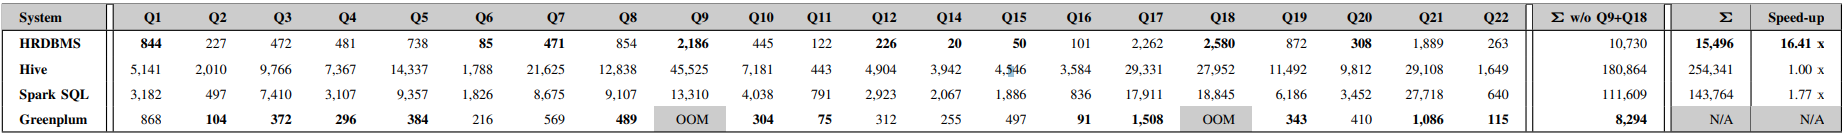
\includegraphics[scale=0.43]{images/test1.png}}
\captionsetup{font=Large}
\caption{Kết quả thực thi trong 8 node \cite{arnold2019hrdbms}}
\label{fig:test1}
\end{table}


Các cột trong bảng:
Q1 - Q22: Thời gian thực thi của các truy vấn TPC-H (được đo bằng mili giây) trên mỗi hệ thống DBMS.

$\Sigma$ w/o Q9+Q18: Tổng thời gian thực thi của tất cả các truy vấn, trừ Q9 và Q18, trên mỗi hệ thống quản lý cơ sở dữ liệu (DBMS).

$\Sigma$: Tổng thời gian thực thi của tất cả các truy vấn trên mỗi hệ thống DBMS.

Speed-up: Chỉ số tăng tốc so với Hive, được tính bằng tổng thời gian thực thi của Hive chia cho tổng thời gian thực thi của mỗi hệ thống DBMS.

Bảng \ref{fig:test1} so sánh hiệu năng này cho thấy sự khác biệt rõ rệt giữa các hệ thống quản lý cơ sở dữ liệu (DBMS) khi thực hiện các truy vấn TPC-H. Dưới đây là đánh giá của mỗi hệ thống dựa trên bảng này:
HRDBMS có hiệu năng xuất sắc so với các hệ thống DBMS khác. Tổng thời gian thực thi của HRDBMS là 15.496 ms, nhanh hơn rất nhiều so với Hive và Spark SQL. Chỉ số tăng tốc của HRDBMS so với Hive là 16,41, cho thấy nó hoạt động nhanh hơn 16,41 lần. HRDBMS thực hiện tốt hơn trong hầu hết các truy vấn và đặc biệt nổi bật trong truy vấn Q9 và Q18.
Hive là hệ thống DBMS chậm nhất trong bảng so sánh này, với tổng thời gian thực thi là 254.341 ms và chỉ số tăng tốc là 1 (được sử dụng làm tiêu chuẩn so sánh). Hive thực hiện chậm nhất trong các truy vấn Q9 và Q18, mất 45.525 ms và 27.952 ms tương ứng.
Spark SQL có hiệu năng tốt hơn Hive nhưng thấp hơn HRDBMS. Tổng thời gian thực thi của Spark SQL là 143.764 ms, và chỉ số tăng tốc so với Hive là 1,77. Spark SQL thực hiện truy vấn Q9 và Q18 với thời gian tương đối nhanh, chỉ mất 13.310 ms và 18.845 ms.
Greenplum có hiệu năng tốt hơn Hive trong một số truy vấn, nhưng không thể hoàn thành truy vấn Q9 do hết bộ nhớ (Out Of Memory - OOM). Do đó, không có số liệu tổng thời gian thực thi và chỉ số tăng tốc cho Greenplum. 

Trên cơ sở bảng \ref{fig:test1} thì HRDBMS là hệ thống DBMS có hiệu năng tốt nhất khi thực hiện các truy vấn TPC-H.

\subsection{Các phương pháp nghiên cứu }
    
Các phương pháp nghiên cứu bao gồm:

\begin{itemize}
\item Xác định vấn đề nghiên cứu: Dựa trên kiến thức lý thuyết về HRDBMS và kết quả phân tích, xác định vấn đề cụ thể, thực tế và có ý nghĩa về quản lý và truy vấn dữ liệu lớn để tập trung nghiên cứu và giải quyết.
\item Chuẩn bị các phần mềm và tập dữ liệu dùng để so sánh: Thực hiện cài đặt và cấu hình các công cụ được sử dụng trong lĩnh vực xử lý và quản lý dữ liệu, nhằm mục đích đối chiếu với HRDBMS gồm Apache Hive, Spark SQL và Greenplum. Sử dụng các tập dữ liệu tổng hợp từ TPC-H làm tiêu chuẩn để đánh giá và so sánh.
\item Thiết lập môi trường thử nghiệm trên các dịch vụ đám mây: Đăng ký và sử dụng các dịch vụ đám mây như Amazon Web Services (AWS) và Google Cloud Platform (GCP) để triển khai và thiết lập môi trường thử nghiệm, bao gồm việc cài đặt và cấu hình các máy chủ ảo, cơ sở dữ liệu HRDBMS và các dịch vụ liên quan khác.
\item Biên dịch, sửa đổi và chạy mã nguồn HRDBMS: Tiến hành biên dịch, sửa đổi và chạy mã nguồn trên môi trường phù hợp.
\item Đề xuất giải pháp và phương pháp giải quyết: Đưa ra các giải pháp và phương pháp giải quyết vấn đề nghiên cứu, bao gồm cải tiến thuật toán, tối ưu hóa hiệu suất, độ tin cậy, khả năng mở rộng, vv. của HRDBMS.
\item Thực nghiệm và kiểm chứng: Thiết kế và triển khai các mô phỏng để kiểm chứng tính hiệu quả, độ tin cậy và khả năng mở rộng của các giải pháp đề xuất cho HRDBMS. Thu thập, phân tích và đánh giá kết quả thực nghiệm để rút ra nhận xét.
\item Viết tài liệu hướng dẫn cài đặt và vận hành giải pháp HRDBMS.
\item Viết luận văn tổng kết lại toàn bộ quá trình và kết quả của việc áp dụng HRDBMS
\end{itemize}


\subsection{Nội dung và phạm vi của vấn đề sẽ đi sâu nghiên cứu}
\begin{itemize}
\item Bản luận văn hoàn chỉnh, mô tả chi tiết cơ sở lý thuyết và các kết quả thu được từ việc nghiên cứu và áp dụng HRDBMS. Luận văn sẽ bao gồm phân tích, đánh giá và đề xuất các giải pháp mới để cải thiện hiệu suất, độ tin cậy và khả năng mở rộng của hệ thống quản lý cơ sở dữ liệu phân tán.
\item Mã nguồn của HRDBMS đã được phát triển và tối ưu hóa một cách đáng kể. Mã nguồn này sẽ đảm bảo tính ổn định, hiệu năng cao và khả năng mở rộng tốt của hệ thống khi xử lý các tác vụ quản lý dữ liệu lớn.
\item Dữ liệu từ TPC-H được chỉnh sửa để phục vụ cho việc đánh giá, thử nghiệm và so sánh hiệu suất của các giải pháp đề xuất. Điều này có thể bao gồm việc tạo ra các tập dữ liệu mô phỏng hoặc sử dụng các tập dữ liệu thực tế từ các nguồn như TPC-H.
\item Các tài liệu kỹ thuật hướng dẫn chi tiết về phương pháp tái tạo các sản phẩm nghiên cứu, bao gồm hướng dẫn sử dụng giải pháp HRDBMS được phát triển, phương pháp tiếp cận và triển khai các giải pháp đề xuất trong thực tế, cũng như hướng dẫn cho các nghiên cứu sau này liên quan đến đề tài.
\end{itemize}

\subsection{Nơi thực hiện đề tài nghiên cứu của luận văn}
Khoa Công nghệ thông tin – Trường đại học Khoa học Tự Nhiên – Đại học quốc gia TP.Hồ Chí Minh
    
\subsection{Thời gian thực hiện}

\begin{longtable}{|>{\raggedright\arraybackslash}p{4cm}|>{\raggedright\arraybackslash}p{3cm}|>{\raggedright\arraybackslash}p{3cm}|>{\raggedright\arraybackslash}p{5cm}|}
\hline
\textbf{Công việc} & \textbf{Thời gian bắt đầu} & \textbf{Thời gian kết thúc} & \textbf{Mô tả} \\
\hline
Nghiên cứu lý thuyết và định hướng đề tài & 01/06/2023 & 15/06/2023 & Trong giai đoạn này, sẽ tập trung vào việc đọc và hiểu lý thuyết về HRDBMS và các công nghệ liên quan. Đồng thời, xác định rõ hướng đi cho đề tài. \\
\hline
Chuẩn bị và tìm hiểu các công cụ và dữ liệu cho việc so sánh & 16/06/2023 & 30/06/2023 & Thực hiện cài đặt và cấu hình các công cụ được sử dụng trong lĩnh vực xử lý và quản lý dữ liệu, nhằm mục đích đối chiếu với HRDBMS gồm Apache Hive, Spark SQL và Greenplum và sử dụng các tập dữ liệu tổng hợp từ TPC-H làm tiêu chuẩn để đánh giá và so sánh. \\
\hline
Thiết lập môi trường thử nghiệm & 01/07/2023 & 15/07/2023 & Đăng ký và sử dụng các dịch vụ đám mây như Amazon Web Services (AWS) và Google Cloud Platform (GCP) để triển khai và thiết lập môi trường thử nghiệm, bao gồm việc cài đặt và cấu hình các máy chủ ảo, cơ sở dữ liệu và các dịch vụ liên quan khác. \\
\hline
Chỉnh sửa và vận hành mã nguồn HRDBMS & 01/08/2023 & 31/08/2023 & Tiến hành biên dịch, sửa đổi và chạy mã nguồn trên môi trường phù hợp. \\
\hline
Đưa ra giải pháp và phương pháp giải quyết vấn đề & 01/09/2023 & 30/09/2023 & Đưa ra các giải pháp và phương pháp giải quyết vấn đề nghiên cứu, bao gồm cải tiến thuật toán, tối ưu hóa hiệu suất, độ tin cậy, khả năng mở rộng, vv. \\
\hline
Tiến hành thử nghiệm và đánh giá kết quả & 01/10/2023 & 31/10/2023 & Thiết kế và triển khai các mô phỏng để kiểm chứng tính hiệu quả, độ tin cậy và khả năng mở rộng của các giải pháp đề xuất. Thu thập, phân tích và đánh giá kết quả thực nghiệm \\
\hline
Soạn thảo, chỉnh sửa và hoàn thiện luận văn & 01/11/2023 & 01/12/2023 & Tập trung vào việc viết và chỉnh sửa bản luận văn, mô tả chi tiết cơ sở lý thuyết và các kết quả thu được từ nghiên cứu, bao gồm phân tích, đánh giá và đề xuất các giải pháp mới cho hệ thống. \\
\hline
\end{longtable}


    





\tableofcontents % Tạo mục lục


\addcontentsline{toc}{section}{Chương 4: NỘI DUNG THỰC HIỆN LUẬN VĂN}
















    
\section{NỘI DUNG THỰC HIỆN LUẬN VĂN}
    {
    
\subsection{Mở đầu}
Trong thời đại kỹ thuật số hiện nay, dữ liệu đóng vai trò quan trọng trong hầu hết mọi khía cạnh của công nghệ thông tin. Đặc biệt, trong các hệ thống quản lý thành viên trực tuyến như ASP.NET Membership database, việc xử lý và quản lý dữ liệu lớn trở thành một thách thức đáng kể. MS SQL Server, một hệ quản trị cơ sở dữ liệu quan hệ phổ biến, đã được sử dụng rộng rãi trong việc quản lý dữ liệu này. Tuy nhiên, với sự phát triển nhanh chóng của dữ liệu và yêu cầu ngày càng cao về hiệu suất và khả năng mở rộng, MS SQL Server bắt đầu cho thấy những hạn chế của mình.

Khi đối mặt với lượng dữ liệu ngày càng tăng, MS SQL Server thường xuất hiện một số vấn đề nghiêm trọng ảnh hưởng đến hiệu suất và khả năng mở rộng. Đầu tiên và rõ ràng nhất là vấn đề tốc độ truy vấn chậm. Trong bối cảnh dữ liệu lớn, việc tìm kiếm và xử lý dữ liệu trở nên phức tạp và tốn thời gian, đặc biệt với các truy vấn liên kết nhiều bảng và có nhiều điều kiện. Điều này không chỉ gây trở ngại cho quá trình truy xuất dữ liệu mà còn làm giảm trải nghiệm người dùng cuối.

Một vấn đề khác là quản lý tài nguyên và bộ nhớ không hiệu quả. MS SQL Server có thể không tối ưu hóa việc sử dụng bộ nhớ và tài nguyên máy chủ khi phải đối phó với lượng lớn giao dịch và dữ liệu. Các vấn đề như sự phân mảnh (fragmentation) của dữ liệu và quản lý bộ nhớ cache không hiệu quả có thể xuất hiện, làm tăng độ trễ trong việc truy cập dữ liệu và ảnh hưởng đến hiệu suất tổng thể.

Ngoài ra, MS SQL Server cũng gặp phải hạn chế về khả năng mở rộng. Trong mô hình truyền thống, việc mở rộng quy mô cơ sở dữ liệu, đặc biệt là mở rộng ngang, không phải lúc nào cũng dễ dàng hoặc kinh tế. Việc tăng cường cơ sở hạ tầng có thể đòi hỏi đầu tư lớn và làm phức tạp quá trình quản lý dữ liệu, đặc biệt là trong các hệ thống cần xử lý lượng lớn dữ liệu liên tục và đồng thời.

Chính những hạn chế này đã tạo ra nhu cầu cấp thiết cho một giải pháp thay thế, và đây là lúc cơ sở dữ liệu phân tán bước vào. Với khả năng mở rộng linh hoạt, quản lý hiệu quả tài nguyên và bộ nhớ, cùng với việc giảm thiểu độ trễ trong xử lý truy vấn nhờ vào cơ chế phân phối dữ liệu qua nhiều nút, cơ sở dữ liệu phân tán trở thành một giải pháp hấp dẫn và hiệu quả hơn trong việc xử lý các thách thức của dữ liệu lớn.

Trong bối cảnh này, cơ sở dữ liệu phân tán đưa ra một giải pháp hứa hẹn. Khác biệt so với mô hình truyền thống, cơ sở dữ liệu phân tán có thể phân chia và quản lý dữ liệu trên nhiều máy chủ, giúp giảm tải cho từng hệ thống và tăng cường hiệu suất tổng thể. Điều này không chỉ giúp giảm độ trễ trong truy vấn mà còn cung cấp khả năng mở rộng và bảo mật dữ liệu tốt hơn.

Mục tiêu của luận văn này là khám phá và phân tích sâu rộng về việc chuyển đổi từ MS SQL Server sang cơ sở dữ liệu phân tán, nhằm giải quyết các vấn đề liên quan đến quản lý dữ liệu lớn trong ASP.NET Membership database. Bằng cách này, nghiên cứu nhằm đề xuất một giải pháp có thể cải thiện đáng kể hiệu suất, khả năng mở rộng, và độ tin cậy của hệ thống quản lý dữ liệu.

Nghiên cứu này không chỉ có ý nghĩa với các nhà phát triển và quản trị viên hệ thống mà còn đóng góp vào lĩnh vực nghiên cứu cơ sở dữ liệu. Kết quả từ nghiên cứu này có thể được áp dụng rộng rãi trong các hệ thống quản lý dữ liệu lớn khác, đặc biệt trong các ứng dụng web hiện đại yêu cầu cao về hiệu suất và khả năng mở rộng.

\subsection{Cơ sở lý thuyết}
Đầu tiên Microsoft SQL Server là một hệ thống quản lý cơ sở dữ liệu quan hệ (RDBMS) phát triển bởi Microsoft. Nó là một giải pháp dữ liệu toàn diện, cung cấp các công cụ và dịch vụ hỗ trợ quản lý, lưu trữ và xử lý dữ liệu trong môi trường doanh nghiệp. SQL Server bao gồm nhiều tính năng và công cụ hỗ trợ, từ quản lý dữ liệu quan hệ và thực hiện truy vấn SQL, đến phân tích dữ liệu, báo cáo và tích hợp dữ liệu.

SQL Server được thiết kế để đáp ứng nhu cầu đa dạng của doanh nghiệp, bao gồm xử lý giao dịch trực tuyến (OLTP), hệ thống hỗ trợ quyết định (DSS), và cung cấp khả năng mở rộng và hiệu suất cao cho cơ sở dữ liệu lớn. Nó cũng đặc biệt mạnh mẽ trong việc đảm bảo an toàn và bảo mật dữ liệu, với các tính năng như mã hóa, quản lý quyền truy cập, và các chính sách bảo mật nâng cao.



\begin{figure}
   \centering
    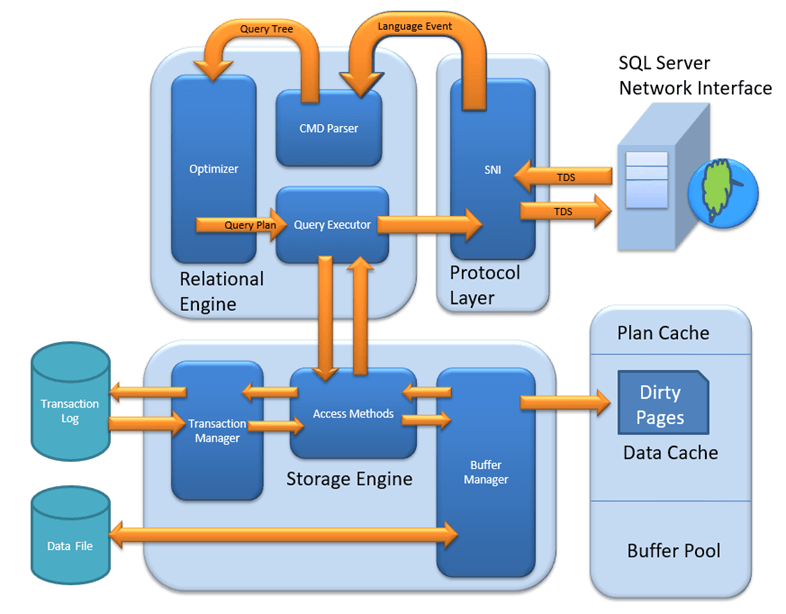
\includegraphics[width=0.5\linewidth]{image1.png}
    \caption{Kiến trúc của Microsoft SQL Server}
    \label{fig:overviewsmssql}
\end{figure}

Hình ảnh \ref{fig:overviewsmssql} được đề cập cung cấp một cái nhìn tổng quan về
kiến trúc của Microsoft SQL Server, Relational Engine đóng vai trò trung tâm trong việc xử lý các truy vấn SQL. Bắt đầu với CMD Parser, nơi mà truy vấn được phân tích cú pháp và chuyển thành một "query tree" – một biểu diễn cấu trúc của các hành động cần thực hiện. Điều này cho phép SQL Server hiểu và chuẩn bị cho việc tối ưu hóa truy vấn.

Tiếp đến là Optimizer, một thành phần chức năng quan trọng của Relational Engine, chịu trách nhiệm cho việc lựa chọn kế hoạch truy vấn hiệu quả nhất từ nhiều lựa chọn có thể. Optimizer xác định chiến lược thực thi dựa trên chi phí tài nguyên như CPU, bộ nhớ và đĩa cứng. Quá trình này đảm bảo rằng truy vấn được thực hiện một cách hiệu quả nhất.

Sau khi kế hoạch được tối ưu hóa, Query Executor bắt đầu công việc của mình, thực thi kế hoạch truy vấn đã được chọn lọc, làm việc cùng với Storage Engine để truy xuất, cập nhật hoặc xóa dữ liệu cần thiết từ cơ sở dữ liệu.

Vai trò của Storage Engine trong kiến trúc này cũng cực kỳ quan trọng. Nó quản lý việc lưu trữ và truy xuất dữ liệu từ đĩa cứng thông qua các phương pháp truy cập dữ liệu. Trong khi đó, Transaction Manager giữ vai trò quản lý các giao dịch, đảm bảo rằng mọi thay đổi dữ liệu đều theo dõi được và có thể khôi phục nếu cần.

Buffer Manager là một phần khác của Storage Engine, quản lý bộ nhớ đệm nơi trang dữ liệu được lưu giữ tạm thời trước khi ghi ra đĩa hoặc sau khi đọc từ đĩa. Quản lý này giúp tối ưu hóa truy cập dữ liệu và tăng cường hiệu suất I/O.

SQL Server còn có SQL Server Network Interface (SNI), cung cấp giao tiếp mạng giữa server và client sử dụng giao thức TDS (Tabular Data Stream), đây là giao thức mạng đặc biệt của SQL Server.

Trong khi Protocol Layer quản lý gói tin TDS giữa client và server, đảm bảo thông tin được truyền đi chính xác và hiệu quả, Buffer Pool gồm Plan Cache và Data Cache đóng một vai trò quan trọng trong việc cải thiện hiệu suất bằng cách lưu giữ các kế hoạch truy vấn và dữ liệu thường xuyên được truy cập. Ngoài ra, Dirty Pages là những trang dữ liệu đã thay đổi trong bộ nhớ đệm và chờ được ghi ra đĩa.

Cuối cùng, Transaction Log ghi lại tất cả các thay đổi dữ liệu để hỗ trợ phục hồi dữ liệu, trong khi các Data File lưu trữ dữ liệu thực tế của cơ sở dữ liệu. Đây là các file vật lý chứa thông tin cần thiết để bảo quản và bảo mật dữ liệu.

Kiến trúc này minh họa một cách chi tiết cách mà SQL Server xử lý các truy vấn từ khi chúng được gửi tới cho đến khi kết quả được trả về, đồng thời duy trì hiệu suất và độ tin cậy.

Microsoft SQL Server là một hệ thống quản lý cơ sở dữ liệu quan hệ vững chắc và được ưa chuộng trên toàn cầu. Tuy nhiên, như mọi hệ thống công nghệ thông tin, nó không phải là không có điểm yếu. Một trong những thách thức lớn nhất mà SQL Server đối mặt là khi xử lý các bộ dữ liệu lớn và phức tạp, đặc biệt trong môi trường có yêu cầu cao về phân tích dữ liệu và báo cáo thời gian thực. Các vấn đề có thể bao gồm chậm chạp trong truy vấn, thời gian chờ (timeouts), và khó khăn trong việc mở rộng quy mô cơ sở dữ liệu.

Trong khi SQL Server có thể xử lý tốt các tải trọng dữ liệu trung bình và lớn, nó không được thiết kế từ đầu để làm việc hiệu quả với cơ sở dữ liệu kích thước rất lớn (big data) hoặc xử lý phân tích song song đại trà (massively parallel processing - MPP). Đây là nơi mà các hệ thống như Greenplum Database bước vào.

Greenplum Database là một RDBMS mã nguồn mở được xây dựng dựa trên PostgreSQL và được thiết kế để chạy trên kiến trúc MPP, cho phép nó xử lý và phân tích lượng dữ liệu lớn một cách nhanh chóng và hiệu quả. Greenplum có khả năng phân phối và xử lý dữ liệu trên nhiều nút và máy chủ khác nhau, giảm đáng kể vấn đề về thời gian chờ và cải thiện đáng kể hiệu suất so với các hệ thống không được thiết kế để mở rộng quy mô theo cách này.

Greenplum có những đặc trưng sau:

Greenplum sử dụng kiến trúc Massively parallel processing (MPP): MPP là một
cách xử lý dữ liệu mà trong đó nhiều bộ vi xử lý thực hiện các tác vụ
khác nhau đồng thời. Điều này giúp xử lý dữ liệu lớn hoặc phức tạp
một cách nhanh chóng và hiệu quả. MPP thường được sử dụng trong
các máy chủ lớn và các hệ thống cơ sở dữ liệu, nơi mà việc xử lý song
song có thể cải thiện đáng kể tốc độ và hiệu suất.
Mỗi máy chủ hoạt động như một "segment" tự chứa, xử lý một phần
của dữ liệu và truy vấn một cách độc lập.Cấu trúc này giúp giảm độ trễ và tăng hiệu suất tổng thể bằng cách
song song hóa các tác vụ, đặc biệt quan trọng khi xử lý các tác vụ đòi
hỏi nhiều tài nguyên tính toán.

Tối ưu hóa cho Online Transaction Processing (OLTP) và OLAP: Tiết kiệm chi phí và đơn giản hóa kiến trúc IT: Do khả năng xử lý cả
OLTP và OLAP trên cùng một hệ thống, Greenplum giúp doanh
nghiệp giảm thiểu sự cần thiết của việc duy trì nhiều hệ thống, từ đó
tiết kiệm chi phí và giảm bớt độ phức tạp của hạ tầng. Giao thức cam kết một pha (One-Phase Commit Protocol): Đối với
các giao dịch chỉ ảnh hưởng đến dữ liệu trên một phân đoạn đơn lẻ
của Greenplum, hệ thống sử dụng giao thức cam kết một pha thay vì
hai pha thông thường. Giao thức hai pha (two-phase commit protocol) là một cơ chế đồng bộ
hóa dùng trong các hệ thống phân tán để đảm bảo rằng tất cả thay đổi
trong một giao dịch được cam kết (commit) một cách đồng nhất trên
tất cả các node hệ thống. Giao thức một pha loại bỏ bước thứ hai,
giảm độ phức tạp và thời gian xử lý cho những giao dịch đơn giản, từ
đó cải thiện hiệu suất và đáp ứng nhanh chóng hơn cho các yêu cầu
OLTP

Khả năng mở rộng Greenplum có thể mở rộng theo chiều ngang bằng cách thêm node vào cụm mà không làm gián đoạn dịch vụ. Khả năng mở rộng này cho phép Greenplum tăng cường nhanh chóng năng lực xử lý khi lượng dữ liệu tăng lên.
Các công cụ này giúp đơn giản hóa việc phân tích dữ liệu phức tạp và
dự đoán, đem lại giá trị từ dữ liệu lớn.

Ngoài việc xử lý các truy vấn SQL cơ bản, Greenplum còn hỗ trợ các
công cụ phân tích dữ liệu nâng cao như machine learning và xử lý dữ
liệu lớn


Những đặc trưng này, khi kết hợp, tạo nên một hệ thống mạnh mẽ, linh hoạt,
và hiệu quả cho việc xử lý khối lượng dữ liệu lớn, đáp ứng cả nhu cầu xử lý
giao dịch hàng ngày và phân tích dữ liệu chuyên sâu.



Nghiên cứu và cài đặt hệ thống Greenplum với mỗi node có hiệu suất tương
đương cơ sở dữ liệu Massively Parallel Processing (MPP) kiến trúc của hệ
thống. Hình \ref{fig:gp-architecture} mô tả kiến trúc của Greenplum.

\begin{figure}[htbp]
\centerline{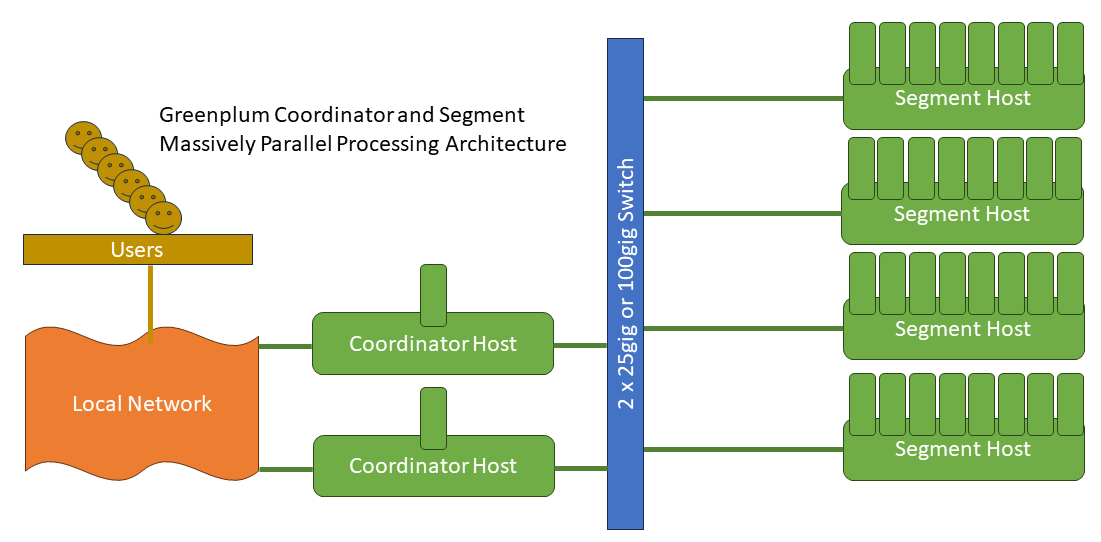
\includegraphics[scale=.4]{images/gp-architecture.png}}
\captionsetup{font=Large}
\caption{Kiến trúc hệ thống cơ sở dữ liệu Greenplum. \cite{vmware_greenplum}. }
\label{fig:gp-architecture}
\end{figure}

Greenplum là hệ thống cơ sở dữ liệu được xây dựng dựa trên kiến
trúc MPP, được tối ưu hóa để xử lý dữ liệu lớn và phân tích. Nó sử dụng kiến
trúc shared-nothing, nơi mỗi node trong hệ thống là độc lập và tự cung cấp tài nguyên cho chính mình, từ CPU, bộ nhớ đến lưu trữ.

Các thành phần chính của kiến trúc Greenplum:

Coordinator trong kiến trúc Greenplum là nơi quản lý và điều phối
toàn bộ hoạt động của cơ sở dữ liệu. Hình \ref{fig:admin_guide-graphics-standby_coordinator} Mô tả coordinator trong kiến trúc Greenplum.
Dưới đây là các yếu tố cụ thể:


\begin{figure}[htbp]
\centerline{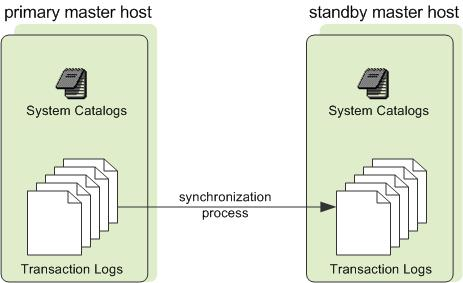
\includegraphics[scale=.7]{images/admin_guide-graphics-standby_coordinator.jpg}}
\captionsetup{font=Large}
\caption{Coordinator trong kiến trúc Greenplum \cite{vmware_greenplum}.}
\label{fig:admin_guide-graphics-standby_coordinator}
\end{figure}

Quản lý truy vấn và điều phối: Coordinator nhận các truy vấn từ ứng dụng người dùng và chịu trách nhiệm phân tích cú pháp, tối ưu hóa truy vấn, và lập kế hoạch thực thi truy vấn. Nó phân phối các phần của truy vấn đã được tối ưu hóa đến các segment nodes để thực hiện.


Duy trì Metadata: Coordinator duy trì danh mục (catalog) của cơ sở dữ liệu, nơi lưu giữ thông tin về sơ đồ, dữ liệu, và cấu trúc của các bảng, cũng như các thông tin thống kê cần thiết cho việc tối ưu hóa truy vấn.

Quản lý giao dịch: Coordinator xử lý và quản lý các giao dịch, đảm bảo tính toàn vẹn, nhất quán, và cô lập dữ liệu. Nó sử dụng giao thức cam kết hai pha (two-phase commit protocol) để đảm bảo các thay đổi được thực hiện một cách đồng nhất trên tất cả các segment nodes.

Quản lý giao dịch: Coordinator xử lý và quản lý các giao dịch, đảm bảo tính toàn vẹn, nhất quán, và cô lập dữ liệu. Nó sử dụng giao thức cam kết hai pha (two-phase commit protocol) để đảm bảo các thay đổi được thực hiện một cách đồng nhất trên tất cả các segment nodes.

Quản lý Tài nguyên: Coordinator quản lý các nguồn tài nguyên như bộ nhớ và CPU cho các truy vấn và có thể thiết lập các ưu tiên dựa trên chính sách quản lý tài nguyên.

Phục hồi và Sao lưu: Trong trường hợp có sự cố, master host có trách nhiệm khởi tạo các quy trình sao lưu và phục hồi để bảo đảm tính sẵn sàng và liên tục của hệ thống.

Monitoring và Logging: Coordinator cũng có trách nhiệm giám sát hoạt động của cả hệ thống và ghi lại các sự kiện hệ thống, giúp trong việc phân tích hiệu suất và khắc phục sự cố. Coordinator đóng vai trò trung tâm trong kiến trúc Greenplum, đảm nhiệm nhiều chức năng quan trọng từ việc quản lý truy vấn đến quản lý tài nguyên và đảm bảo tính ổn định của hệ thống.

Trong kiến trúc Greenplum, segment là những máy chủ cơ sở dữ liệu hoặc
"nodes" làm việc song song để xử lý và lưu trữ dữ liệu. Dưới đây là mô tả chi tiết về segment trong Greenplum:

Xử lý dữ liệu song song: Mỗi segment là một node xử lý độc lập, chạy một instance của cơ sở dữ liệu PostgreSQL. Các segment làm việc cùng nhau một cách song song, mỗi segment xử lý một phần của truy vấn tổng thể và dữ liệu liên quan.

Lưu trữ phân tán: Dữ liệu trong Greenplum được phân phối đều ra các segment. Mỗi segment chứa một phần dữ liệu và được quản lý độc lập.
Kỹ thuật phân phối có thể bao gồm hash-based, random, hoặc các phân vùng
dữ liệu cụ thể. 

Tính độc lập và kiến trúc shared-nothing:
Mỗi segment có bộ nhớ và không gian lưu trữ của riêng mình, tuân theo kiến trúc shared-nothing. Điều này đảm bảo rằng không có sự phụ thuộc giữa các segment, giảm thiểu các điểm nghẽn và cải thiện hiệu suất.

Tự động phục hồi: Greenplum có khả năng tự động phục hồi từ lỗi ở cấp segment. Khi một segment gặp sự cố, Greenplum có thể chuyển công việc sang một segment dự bị hoặc phục hồi segment bị lỗi.

Hiệu suất cao và khả năng mở rộng: Do mỗi segment xử lý một phần nhỏ của dữ liệu, hệ thống có thể mở rộng quy mô một cách linh hoạt bằng cách thêm segment vào hệ thống để xử lý khối lượng dữ liệu lớn hơn.
Sự mở rộng này có thể được thực hiện mà không cần thay đổi cấu trúc hoặc
cấu hình của các segment hiện có.

Quản lý và giám sát:
Mỗi segment được giám sát bởi coordinator, đảm bảo rằng nó hoạt động đúng
và hiệu quả. Coordinator có thể giám sát tình trạng và hiệu suất của từng segment, và thực hiện các điều chỉnh khi cần thiết.

Cân bằng tải: Greenplum sử dụng cơ chế cân bằng tải để đảm bảo rằng không có segment nào bị quá tải hoặc nhàn rỗi.
Việc phân phối công việc giữa các segment được thực hiện dựa trên cấu hình và tình trạng hiện tại của hệ thống.

Segments đóng vai trò quan trọng trong việc đảm bảo khả năng xử lý dữ liệu lớn và phức tạp của Greenplum, giúp nó trở thành một giải pháp mạnh mẽ cho việc kho dữ liệu và phân tích dữ liệu quy mô lớn.

Greenplum đã giới thiệu một node kế hoạch mới có tên là Motion để thực hiện việc di chuyển dữ liệu này. Node Motion sử dụng mạng để gửi và nhận dữ liệu từ các segment khác nhau, tạo điều kiện cho việc phân chia kế hoạch truy vấn thành nhiều phần khác nhau, mỗi phần được gọi là một "slice". Mỗi slice sau đó được thực thi bởi một nhóm các quá trình phân tán, được gọi chung là "gang". Với việc sử dụng node Motion và khái niệm gang, kế hoạch truy vấn và quá trình thực thi của Greenplum trở nên phân tán. Kế hoạch sẽ được gửi đến từng quá trình, và mỗi quá trình sẽ thực thi phần slice của kế hoạch dựa trên ngữ cảnh và trạng thái cục bộ của mình. Điều này phản ánh kỹ thuật Single Program Multiple Data (SPMD), nơi cùng một kế hoạch được phân phát đến các nhóm quá trình trên khắp cụm. Các quá trình khác nhau được tạo ra bởi các segment khác nhau sẽ có ngữ cảnh, trạng thái và dữ liệu cục bộ riêng của chúng. Hình \ref{fig:plan} ví dụ về kế hoạch phân tán và thực thi của Greenplum.

\begin{figure}[htbp]
\centerline{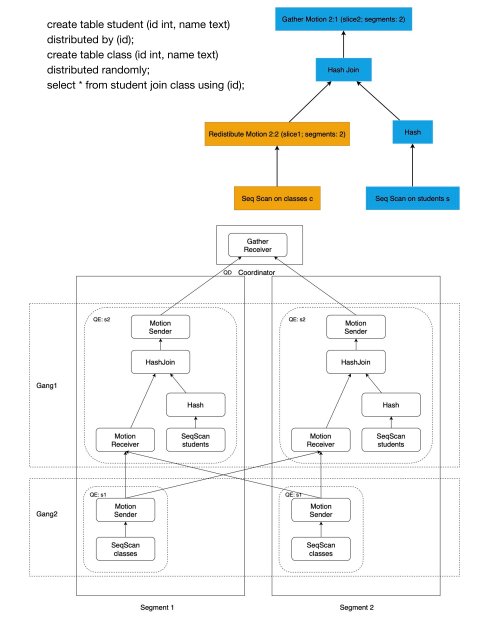
\includegraphics[scale=.8]{images/plan.PNG}}
\captionsetup{font=Large}
\caption{Kế hoạch phân tán và thực thi của Greenplum \cite{lyu2021greenplum}}
\label{fig:plan}
\end{figure}

Từ hình \ref{fig:plan} cho thấy Greenplum bảng student được tạo với việc phân phối dữ liệu dựa trên cột id. Điều này có nghĩa là dữ liệu sẽ được phân chia giữa các segment sao cho mỗi id student sẽ chỉ tồn tại trên một segment cụ thể. Bảng class được tạo với dữ liệu phân phối một cách ngẫu nhiên, không theo một quy tắc cụ thể nào. Khi truy vấn "SELECT * FROM student JOIN class USING (id);" được thực hiện, hệ thống sẽ tạo ra một kế hoạch thực thi phân tán. Kế hoạch này xác định làm thế nào dữ liệu từ cả hai bảng sẽ được kết hợp dựa trên cột id. Các segment thực hiện quét tuần tự (Seq Scan) trên bảng student và class để lấy các bản ghi cần thiết cho việc thực hiện join. Motion Sender: Nằm trên mỗi Motion Sender: Nằm trên mỗi segment, sẽ xác định các bản ghi từ bảng
class mà cần được di chuyển để join với bảng student.
Motion Receiver nằm trên segment đích, sẽ nhận các bản ghi từ bảng class
đã được gửi qua và chuẩn bị cho việc join, sẽ xác định các bản ghi từ bảng class mà cần được di chuyển để join với bảng student. Motion Receiver nằm trên segment đích, sẽ nhận các bản ghi từ bảng class đã được gửi qua và chuẩn bị cho việc join. Trong mỗi segment, một "Hash Join" được thực hiện giữa các bản ghi từ bảng student và các bản ghi từ bảng class đã được di chuyển đến. Đây là bước dữ liệu từ bảng class có thể cần được phân phối lại (redistributed) giữa các phân đoạn để đảm bảo rằng mỗi student có thể được join với đúngclass dựa trên id. Sau khi join được thực hiện trên các phân đoạn, kết quả sau cùng sẽ được gửi về cho "Gather Receiver" ở coordinator, nơi tất cả kết quả từ các phân đoạn được tổng hợp lại. Coordinator sau đó sẽ trả về kết quả cuối cùng của truy vấn join cho người dùng hoặc ứng dụng đã yêu cầu truy vấn. Trong quá trình này, "Gang1" và "Gang2" có thể hiểu là nhóm các quá trình làm việc trên các phân đoạn khác nhau để thực hiện các phần khác nhau của kế hoạch thực thi (ví dụ: quét tuần tự, join). Mỗi "gang" có thể gồm nhiều "slice", tương ứng với một phần của công việc cần thực hiện trên mỗi phân
đoạn.

Trong Greenplum, khóa được sử dụng rộng rãi để ngăn chặn các tình huống
đua tranh ở nhiều cấp độ khác nhau. Có ba loại khóa khác nhau được thiết kế cho các trường hợp sử dụng khác nhau: khóa quay vòng (spin locks), khóa nhẹ (LWlocks), và khóa đối tượng (Object locks).

Khóa quay vòng là loại khóa cực kỳ đơn giản, thường được sử dụng để bảo
vệ các cấu trúc dữ liệu nhỏ và đơn giản. Khi một tiến trình cần truy cập vào một tài nguyên được bảo vệ bởi một spin lock, nó sẽ liên tục kiểm tra (hay "quay vòng") để xem khóa có sẵn hay không. Nếu khóa không sẵn có, tiến trình sẽ tiếp tục vòng lặp này cho đến khi nó có thể giành được khóa. Spin locks phù hợp khi thời gian giữ khóa ngắn, vì nó yêu cầu tiến trình tiêu tốn CPU cho việc quay vòng kiểm tra khóa. Nếu một tiến trình giữ spin lock trong thời gian dài, nó có thể gây ra hiệu suất kém vì các tiến trình khác sẽ phải chờ đợi trong vòng lặp quay vòng.
LWlocks phức tạp hơn spin locks và thường được sử dụng để bảo vệ các cấu
trúc dữ liệu lớn hơn hoặc các hoạt động phức tạp hơn. Chúng cho phép một
số mức độ đọc hoặc viết song song, và cung cấp một cơ chế chờ đợi hiệu quả
hơn so với việc quay vòng liên tục. Khi một tiến trình cần một LWlock nhưng không thể lấy được ngay lập tức, nó sẽ đi vào trạng thái chờ đợi thay vì quay vòng. Điều này giúp giảm tải cho CPU và cho phép xử lý các tiến trình khác trong khi đang chờ.

Khóa đối tượng: Là một cơ chế khóa ở cấp độ cao, được sử dụng để quản lý
truy cập và cập nhật trên các đối tượng cơ sở dữ liệu như bảng, bản ghi, và giao dịch. Đảm bảo rằng nhiều quá trình có thể đồng thời làm việc trên cùng một cơ sở dữ liệu mà không làm ảnh hưởng đến tính toàn vẹn và nhất quán của dữ liệu. Truy cập song song: Khi nhiều quá trình cần truy cập hoặc thao tác trên cùng một đối tượng, khóa đối tượng sẽ quản lý cách thức và mức độ mà mỗi quá trình có thể tương tác với đối tượng đó.

Bảng \ref{tab:khoadoituong} mô tả các cấp độ khóa trong khóa đối tượng: 

\begin{longtable}{|>{\raggedright\arraybackslash}p{6cm}|>{\raggedright\arraybackslash}p{1cm}|>{\raggedright\arraybackslash}p{2cm}|>{\raggedright\arraybackslash}p{2cm}|>{\raggedright\arraybackslash}p{5cm}|}
\hline
\textbf{Tên khóa} & \textbf{Mức độ} & \textbf{Xung đột} & \textbf{Lệnh} &\textbf{Mô tả}\\ 
\hline
AccessShareLock & 1 & 8 & select & Đây là chế độ khóa nhẹ nhất, thường được sử dụng cho các lệnh đọc dữ liệu không thay đổi dữ liệu (như SELECT). Nó chỉ xung đột với chế độ khóa cao nhất, AccessExclusiveLock, giúp cho nhiều quá trình có thể đọc cùng một dữ liệu cùng lúc. \\
\hline
RowShareLock  & 2 & 7, 8 & Select for update & Khóa này được áp dụng trong các thao tác SELECT FOR UPDATE. Nó khóa các hàng được chọn để cập nhật nhưng vẫn cho phép các giao dịch khác đọc các hàng này. \\
\hline
RowExclusiveLock & 3 & 5, 6, 7, 8 & Insert & Thường được sử dụng trong các thao tác INSERT. Nó ngăn các giao dịch khác sửa đổi cùng một hàng, nhằm đảm bảo tính toàn vẹn dữ liệu khi chèn. \\
\hline
ShareUpdateExclusiveLock & 4 & 4, 5, 6, 7, 8 & Vacuum (not full) & Thường được sử dụng trong các thao tác bảo trì như VACUUM (không phải toàn bộ). Khóa này hạn chế hơn để tránh xung đột trong các tác vụ bảo trì. \\
\hline
ShareLock & 5& 3, 4, 6, 7, 8 & Create index & Được áp dụng trong các thao tác như CREATE INDEX. Nó hạn chế hơn để bảo vệ cấu trúc của bảng trong khi chỉ mục đang được tạo. \\
\hline
ShareRowExclusiveLock & 6 & 3, 4, 5, 6, 7, 8 & Collation create & Được sử dụng trong các thao tác sửa đổi lược đồ, như tạo collation. Khóa này khá hạn chế để đảm bảo sự nhất quán của các thay đổi lược đồ. \\
\hline
ExclusiveLock & 7 & 2, 3, 4, 5, 6, 7, 8 & Concurrent refresh matview & Áp dụng trong các thao tác như REFRESH MATERIALIZED VIEW CONCURRENTLY. Nó rất hạn chế để ngăn các giao dịch khác thực hiện các thay đổi có thể xung đột với việc làm mới view. \\
\hline
AccessExclusiveLock & 8& 1, 2, 3, 4, 5, 6, 7, 8 & Alter table & Khóa hạn chế nhất, được sử dụng trong các thao tác như ALTER TABLE. Cơ bản nó khóa tất cả các thao tác khác trên bảng để đảm bảo tính toàn vẹn của các thay đổi cấu trúc lớn. \\
\hline
\caption{Mô tả các cấp độ khóa trong khóa đối tượng \cite{lyu2021greenplum}}
\label{tab:khoadoituong}
\end{longtable}

Khóa đối tượng phân biệt giữa các thao tác đọc và ghi, cho phép độc lập trong
truy cập đọc trong khi quản lý cẩn thận truy cập bản ghi để tránh xung đột dữ
liệu.


\subsection{Phát biểu bài toán}

Trong bối cảnh công nghệ thông tin ngày càng phát triển, Microsoft SQL Server (MSSQL) đã trở thành nền tảng không thể thiếu trong việc quản lý và xử lý dữ liệu lớn, đặc biệt là trong các hệ thống quản lý người dùng như ASP.NET Membership. Tuy nhiên, các thách thức về hiệu suất đã trở nên rõ rệt khi hệ thống phải đối mặt với lượng dữ liệu ngày càng tăng. Điều này đặc biệt trở nên nghiêm trọng trong các hệ thống có hàng triệu người dùng, nơi mà MSSQL cần xử lý một lượng lớn các yêu cầu truy vấn phức tạp và dữ liệu liên tục.

Vấn đề này không chỉ dẫn đến sự chậm trễ trong việc xử lý truy vấn, mà còn tạo ra tình trạng hệ thống thường xuyên bị timed out, đặc biệt trong các trường hợp truy vấn dữ liệu lớn hoặc trong giờ cao điểm. Những vấn đề hiệu suất này không chỉ gây ra sự không tin cậy trong hệ thống mà còn ảnh hưởng trực tiếp đến trải nghiệm của người dùng, khiến họ phải đối mặt với thời gian tải trang lâu và trải nghiệm không mượt mà. Đồng thời, khả năng mở rộng và bảo mật của hệ thống cũng trở thành những thách thức đáng kể. Việc mở rộng cơ sở dữ liệu để xử lý hiệu quả lượng dữ liệu ngày càng lớn đòi hỏi phải vượt qua những rào cản về mặt kỹ thuật, trong khi những vấn đề hiệu suất không ổn định có thể làm tăng rủi ro bảo mật, gây ra nguy cơ tổn thương cho hệ thống.

Những thách thức này không chỉ là vấn đề kỹ thuật cần giải quyết mà còn có tác động sâu rộng đến hoạt động kinh doanh và sự phát triển lâu dài của tổ chức. Chính vì vậy, việc tìm kiếm và áp dụng các giải pháp tối ưu hóa hiệu suất MSSQL trong môi trường ASP.NET Membership trở thành một yêu cầu cấp thiết, không chỉ để cải thiện hiệu suất kỹ thuật mà còn để nâng cao sự hài lòng của người dùng và đảm bảo sự ổn định trong quản lý dữ liệu.


Hơn nữa, những vấn đề về hiệu suất không chỉ ảnh hưởng đến người dùng cuối mà còn gây ra những thách thức lớn trong việc mở rộng và bảo mật hệ thống. Khi hệ thống không thể xử lý hiệu quả các yêu cầu ngày càng tăng, khả năng mở rộng để đáp ứng nhu cầu tăng trưởng trở nên hạn chế, làm cản trở sự phát triển của doanh nghiệp. Ngoài ra, hệ thống bị chậm trễ và không ổn định cũng tạo ra các lỗ hổng bảo mật tiềm tàng, đe dọa đến tính bảo mật của dữ liệu quan trọng.


Trong thế giới sôi động của thương mại điện tử, một trang web lớn đang phục vụ hàng triệu khách hàng, nơi hàng ngày diễn ra vô số giao dịch. Được vận hành trên nền tảng ASP.NET Membership và MSSQL, hệ thống này gặp thách thức không nhỏ trong việc quản lý và phân tích lượng dữ liệu khổng lồ từ thông tin khách hàng và giao dịch. Quản trị viên của trang web phải đối mặt với nhiệm vụ đầy thách thức: tổng hợp báo cáo doanh thu hàng tháng và thống kê chi tiết về số lượng khách hàng cùng các giao dịch, yêu cầu xử lý dữ liệu từ nhiều nguồn khác nhau, từ thông tin giao dịch, hành vi mua sắm, đến số lượng sản phẩm bán ra.

Tuy nhiên, quá trình tạo báo cáo này trở nên khó khăn khi quản trị viên phải vật lộn với những vấn đề về hiệu suất của hệ thống. Mỗi lần họ thực hiện truy vấn tổng hợp dữ liệu, hệ thống MSSQL mất nhiều thời gian để xử lý, bởi phải quét qua hàng triệu bản ghi dữ liệu, gây ra độ trễ đáng kể trong việc tải báo cáo. Hơn nữa, trong giờ cao điểm, khi lượng truy cập tăng vọt, các truy vấn lớn và phức tạp thường không được hệ thống xử lý kịp thời, dẫn đến tình trạng thời gian chờ tăng lên. Điều này không chỉ ảnh hưởng đến quản trị viên mà còn tới trải nghiệm của người dùng khác trên trang web. Thêm vào đó, khi cập nhật dữ liệu giao dịch và thông tin người dùng, hệ thống đôi khi gặp phải tình trạng bế tắc, với các truy vấn cạnh tranh nhau để truy cập cùng một tập dữ liệu, làm gián đoạn hoạt động của hệ thống.Một trang web lớn sử dụng ASP.NET Membership và MSSQL phải đối mặt với hàng loạt thách thức đáng kể liên quan đến hiệu suất trong việc xử lý và tổng hợp dữ liệu:

Chậm trễ (Slowness) trong tổng hợp dữ Liệu:
Khi quản trị viên bắt đầu quá trình tổng hợp dữ liệu cho báo cáo, họ phải đối mặt với nhiệm vụ khổng lồ: xử lý hàng triệu bản ghi dữ liệu. Việc thực hiện các truy vấn phức tạp, cần quét qua lượng lớn dữ liệu, dẫn đến thời gian chờ kéo dài bất thường. Kết quả là, thời gian cần thiết để tải và xem báo cáo tăng lên đáng kể, gây ra độ trễ không mong muốn và ảnh hưởng đến quá trình ra quyết định kinh doanh.

Thời gian chờ(timeout) trong giờ cao điểm:
Đặc biệt trong những khoảng thời gian cao điểm của hoạt động kinh doanh, như trong các sự kiện khuyến mãi hoặc mùa lễ, áp lực đối với hệ thống tăng lên đáng kể. Số lượng lớn truy cập cùng lúc và hàng loạt truy vấn đồng thời gửi đến cơ sở dữ liệu gây ra tình trạng quá tải. Hệ thống, dưới sự nặng nề của truy vấn và cập nhật liên tục, thường xuyên rơi vào tình trạng thời gian chờ dài, ảnh hưởng đến hiệu suất tổng thể và trải nghiệm người dùng.

Deadlocks trong xử lý dữ liệu:
Một thách thức khác nổi bật là tình trạng bế tắc trong quá trình xử lý dữ liệu. Khi nhiều truy vấn cùng lúc cố gắng cập nhật hoặc truy xuất thông tin từ cùng một bộ dữ liệu, hệ thống có thể rơi vào trạng thái khóa lẫn nhau. Sự cố này không chỉ làm giảm tốc độ xử lý dữ liệu mà còn có thể gây ra các sự cố nghiêm trọng trong việc cập nhật và duy trì dữ liệu, gây gián đoạn cho các hoạt động của trang web.

Những thách thức này tạo ra một môi trường đầy áp lực cho quản trị viên và đòi hỏi cần phải có giải pháp công nghệ tiên tiến và sáng tạo để xử lý dữ liệu một cách hiệu quả hơn, đảm bảo rằng hệ thống có thể đáp ứng nhanh chóng và chính xác theo nhu cầu kinh doanh và người dùng.




\subsection{Giải pháp đề xuất}
Để giải quyết vấn đề trên(5.3), việc áp dụng một nền tảng dữ liệu song song đóng vai trò quan trọng. Đối mặt với những thách thức về hiệu suất trong việc tổng hợp và phân tích dữ liệu lớn của web thương mại điện tử là triển khai nền tảng dữ liệu song song. Thông qua việc phân tán quy trình xử lý dữ liệu trên một hệ thống các máy chủ và nút, hệ thống không những cải thiện đáng kể tốc độ xử lý dữ liệu mà còn giảm thiểu thời gian chờ xuống mức tối thiểu.

Bằng cách phân tán tải xử lý, các truy vấn dữ liệu lớn và phức tạp, trước đây là nguồn gốc của sự chậm trễ, nay trở nên linh hoạt và nhanh chóng. Điều này không chỉ tối ưu hóa quá trình tổng hợp báo cáo mà còn nâng cao hiệu quả trong việc phân tích dữ liệu. Kết quả là các báo cáo phức tạp từ doanh thu đến xu hướng hành vi khách hàng, giờ đây có thể được tạo ra một cách nhanh chóng và chính xác, mang lại cái nhìn sâu sắc và toàn diện về hoạt động kinh doanh.

Việc áp dụng nền tảng dữ liệu song song thực sự là một bước ngoặt, biến thách thức về dữ liệu lớn thành cơ hội, mở ra cánh cửa mới cho việc phân tích sâu và chi tiết, đồng thời nâng cao hiệu suất và khả năng phục vụ của hệ thống.

Trong bối cảnh cạnh tranh gay gắt của thương mại điện tử hiện đại, việc áp dụng công nghệ Big Data, và cụ thể hơn, việc sử dụng Greenplum trong việc xử lý và phân tích dữ liệu lớn. Greenplum, với khả năng xử lý song song và hiệu suất làm việc ấn tượng, có thể thay thế trong việc giải quyết các thách thức liên quan đến bộ dữ liệu lớn và phức tạp. Hơn nữa, Greenplum mang lại khả năng tạo ra các báo cáo chi tiết và chính xác, cung cấp cái nhìn đa chiều về doanh thu, hành vi khách hàng, và các xu hướng nổi bật trên thị trường.

Xử lý song song và tối ưu hóa hiệu suất: Greenplum sử dụng mô hình xử lý song song, phân chia công việc xử lý dữ liệu lớn thành các tác vụ nhỏ hơn và phân tán chúng qua nhiều nút. Điều này giúp giảm đáng kể thời gian cần thiết để xử lý truy vấn phức tạp, giải quyết vấn đề chậm trễ mà các hệ thống cơ sở dữ liệu truyền thống thường gặp phải.

Khả năng mở rộng linh hoạt: Greenplum cho phép mở rộng cơ sở dữ liệu một cách linh hoạt, hỗ trợ xử lý dữ liệu lớn mà không làm giảm hiệu suất. Điều này đặc biệt quan trọng đối với trang thương mại điện tử, nơi lượng dữ liệu tăng lên nhanh chóng.

Hiệu quả trong việc giảm ghời gian chờ: Nhờ vào khả năng xử lý song song, Greenplum giảm thiểu tình trạng thời gian chờ khi thực hiện các truy vấn lớn, đặc biệt trong những thời điểm cao điểm của trang web.

Phân tích dữ liệu mạnh mẽ: Greenplum không chỉ là một giải pháp lưu trữ dữ liệu mà còn cung cấp công cụ phân tích mạnh mẽ, cho phép trích xuất, hỗ trợ việc phân tích dữ liệu sâu và rộng.

giảm thiểu rủi ro deadlocks: Trong môi trường xử lý song song, Greenplum giảm thiểu rủi ro deadlocks mà các hệ thống truyền thống thường gặp phải khi xử lý nhiều truy vấn cùng một lúc.

Qua việc triển khai Greenplum, trang thương mại điện tử có thể không chỉ tăng cường hiệu suất và giảm thiểu các vấn đề về chậm trễ, thời gian chờ, và deadlocks, mà còn mở ra cơ hội phân tích dữ liệu một cách chi tiết và chính xác, tối ưu hóa quyết định kinh doanh và cải thiện trải nghiệm người dùng.

\subsection{Cài đặt giải pháp}
Bổ sung sau
\subsection{Đánh giá giải pháp}
Bổ sung sau
    
   
    \pagebreak 
    %TÀI LIỆU TRÍCH DẪN
    %Đây là ví dụ
    \bibliographystyle{ieeetr}
    \bibliography{References/references}
    \nocite{*}

    \begin{table}[h]
    \centering
        \begin{tabular}{p{7cm}p{7cm}}
        \textbf{\begin{tabular}[c]{@{}c@{}}\\XÁC NHẬN\\CỦA NGƯỜI HƯỚNG DẪN\\ \textit{(Ký và ghi rõ họ tên)}\end{tabular}} & \textbf{\begin{tabular}[c]{@{}c@{}}\textit{TP. Hồ Chí Minh, ngày... tháng... năm...}\\HỌC VIÊN THỰC HIỆN\\\textit{(Ký và ghi rõ họ tên}) \end{tabular}}
        \end{tabular}
    \end{table}

\end{document}